
\subsection{Sprawdzenie przecinania się wielokątów wypukłych z użyciem zamiatania (7.1)} 
\paragraph{Treść.} Zaprojektuj algorytm, który w 
czasie $O(n)$ sprawdzi, czy dwa zadane wielokąty wypukłe o nie więcej
niż $n$ wierzchołkach się przecinają. 

\paragraph{Rozwiązanie.}
Stosujemy metodę zamiatania. Zdefiniujmy \textit{zdarzenie}
jako typ danych, który przechowuje wierzchołek $p$, dwa
odcinki $s_1$, $s_2$, których końcem jest $p$ oraz informację 
do którego wielokątu należy ten wierzchołek.

Przyjmujemy, że na wejściu oba wielokąty będą
reprezentowane przez listę zdarzeń posortowanych
względem współrzędnej x wierzchołka $p$. 

Stosujemy zmodyfikowaną wersję algorytmu \ref{HasIntersectingSegments1}, który za 
pomocą metody zamiatania stwierdza, czy w podanym
zbiorze odcinków istnieją dwa, które się przecinają.  

Aby scalić dwie wejściowe listy reprezentujące wierzchołki pierwszego
i drugiego wielokąta, możemy zastosować liniową metodę scalania
znaną z algorytmu \textsc{MergeSort}. Taka uporządkowana lista
będzie stanowiła $X$-strukturę.

Jako $Y$-strukturę możemy przyjąć dowolną strukturę danych, która
zapewni możliwość wykonania wymaganych operacji. Ze względu 
na to, że w $Y$-strukturze nie może znaleźć się więcej niż 
4 odcinki jednocześnie (bo każdy wierzchołek jest jednocześnie
końcem jednej krawędzi i początkiem drugiej oraz mamy 
2 wielokąty), możemy przyjąć, że operacje na $Y$-strukutrze wykonują się w czasie $O(1)$.

Jako że sytuację, w której jeden wielokąt znajduje się wewnątrz drugiego
wielokąta również traktujemy jako przecięcie wielokątów, musimy nanieść modyfikację
na algorytm \ref{HasIntersectingSegments1}. Modyfikacja polega na sprawdzeniu, 
czy występuje sytuacja, w której dodany odcinek $s$
jednego wielokąta znajduje się nad odcinkiem $s_1$ oraz pod odcinkiem $s_2$,
które należą do drugiego wielokąta. Z wypukłości wielokątów wiemy, że 
taka sytuacja wystąpi tylko wtedy, gdy wielokąty na siebie nachodzą lub
jeden jest wewnątrz drugiego.
 
\begin{algorithm}[H]
	\caption{Sprawdzenie czy wielokąty się przecinają}
	\begin{algorithmic}[1]
		\Procedure{HasIntersectingSegments}{$S$: zbiór odcinków spełniający założenia}
		\State $X \gets \textsc{Merge}(L_1, L_2)$ 
		\State $Y \gets \emptyset$
		\While{$X \not = \emptyset$}
		\State \textit{zdarzenie} $\gets$ $X.$DetachHead()
		\State $s_1, s_2 \gets \text{odcinki odpowiadające \textit{zdarzeniu}}$
		\State $p \gets \text{punkt odpowiadający \textit{zdarzeniu}}$
		\If{$p$ jest początkiem odcinika $s$}
		\State Dodaj $s$ do $Y$-struktury
		\If {$s$ należy do jednego wielokąta oraz $Y$.Above($s$) lub z $Y$.Below($s$)
		należą do drugiego}
		\State \Return true
		\EndIf
		\If{$s$ przecina się z $Y$.Above($s$) lub z $Y$.Below($s$)}
		\State \Return true
		\EndIf
		\Else
		\If{$Y$.Above($s$) przecina się z $Y$.Below($s$)}
		\State \Return true
		\EndIf
		\EndIf
		\EndWhile
		\State \Return false
		\EndProcedure
	\end{algorithmic}
	\label{algZadanie7_1}
\end{algorithm}

\subsection{Sprawdzenie przynależności punktu do wielokąta (7.3)}
\paragraph{Treść.} Zaprojektuj strukturę danych, która dla zadanego wielokąta bez samoprzecięć o 
$n$ wierzchołkach pozwoli
na sprawdzenie przynależności punktów do tego wielokąta w czasie $O(\log n)$.
Wskazówka: wykorzystaj metodę zamiatania.
\paragraph{Rozwiązanie.} 
Wielokąt opisany jest przez ciąg punktów posortowanych przeciwnie do ruchu wskazówek zegara. W preprocessingu przygotowujemy przechowywanie wierzchołków wielokąta tak, że dla każdego z nich w czasie stałym jesteśmy w stanie określić dwa odcinki, których dany wierzchołek jest krańcem.

Zamiatamy od lewej do prawej. Zdarzenia przechowujemy w tablicy $X$ posortowanej po współrzędnej $x$-owej. W każdym zdarzeniu (napotkaniu punktu) przechowujemy tablicę odcinków znajdujących się w danym momencie w $Y$-strukturze posortowaną po rosnącej współrzędnej $y$-owej. 

Niech $P$ będzie punktem, którego przynależność do wielokąta sprawdzamy. W tablicy $X$ wyszukiwaniem połówkowym szukamy punktu $A$ o największej współrzędnej $x$ takiego, że $x_A < x_P$. Jako $Y_A$ oznaczmy tablicę odcinków odpowiadających zdarzeniu napotkania punktu $A$ (rysunek \ref{fig:zad73}). 

Zauważmy, że punkt $P$ należy do wielokąta wtedy i tylko wtedy, gdy liczby boków wielokąta nad i pod $P$ są nieparzyste (lub $P$ leży na jednym z boków wielokąta). Potrzebujemy zatem znać liczbę odcinków nad i pod $P$ znajdujących się w tablicy $Y_A$. W tym celu ponownie wykorzystujemy wyszukiwanie połówkowe.

Złożoność algorytmu sprawdzania przynależności jest logarytmiczna (nie liczymy preprocessingu wielokąta), ponieważ dwukrotnie używamy wyszukiwania połówkowego.

\begin{figure}[H]
	\centering
	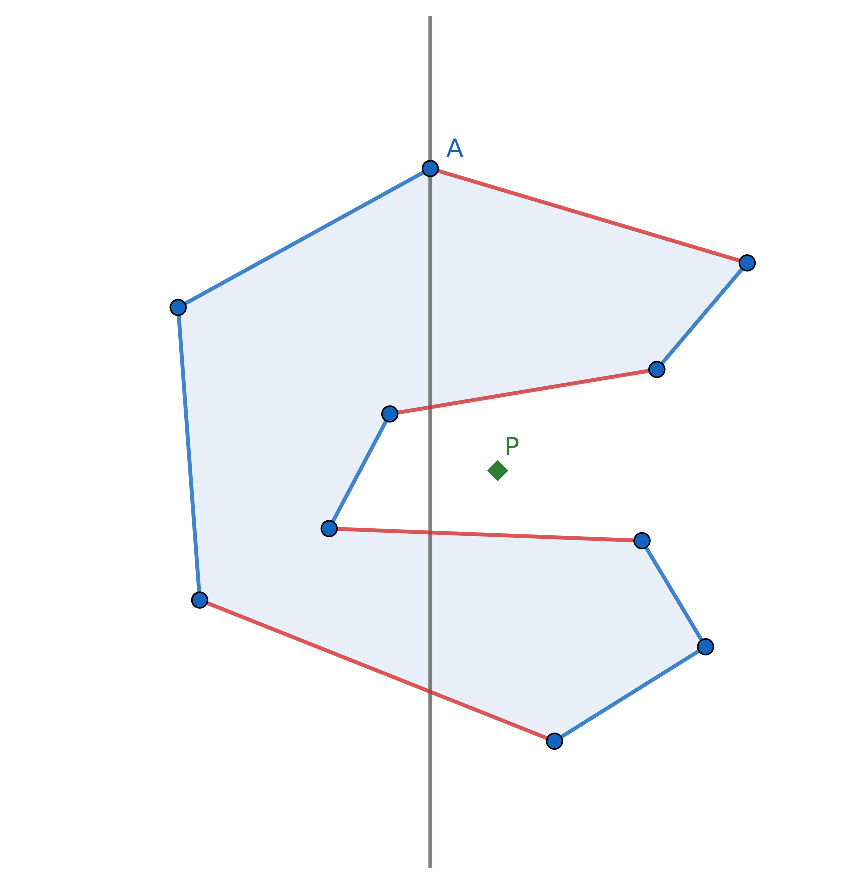
\includegraphics[height=0.45\linewidth]{data/zad73.eps}
	\caption{Punkt $A$ jest najbardziej wysuniętym w prawo punktem położonym na lewo od $P$. Szara prosta reprezentuje miotłę. Na czerwono zaznaczono odcinki znajdujące się w tablicy $Y_A$ (to znaczy obecne w $Y$-strukturze po napotkaniu punktu $A$ przy zamiataniu).}	
	\label{fig:zad73}
\end{figure}

% Algorytm \ref{alg:Zadanie7_1} zakłada, że wielokąt nie ma boków równoległych do osi $OY$ oraz punkt $P$ nie należy do wielokątów . Rozszerzenie algorytmu na 

\begin{algorithm}[H]
	\caption{Sprawdzenie przynależności punktu do wielokąta}
	\begin{algorithmic}[1]
		\Procedure{IsPointInsidePolygon}{$X$: tablica zdarzeń, $P$: punkt}
			\State $A \gets \text{najbardziej wysunięty w prawo punkt położonym na lewo od $P$ (\textit{binary search})}$	
			\State $Y \gets \text{tablica odcinków przechowywana w zdarzeniu napotkania punktu $A$. }$Za początek odcinka przyjmujemy punkt o mniejszej współrzędnej $x$, w przypadku równości o mniejszej współrzędnej $y$.
			\State $a \gets 0$
			\State $b \gets |Y|-1$
			\State 
			
			% Szczerze to nie jestem pewny czy to indeksowanie tutaj działa, chyba tak, ale nie mam siły żeby sprawdzić dokładnie
			\While{$b-a\neq1$}
				\State $i \gets \left\lfloor \frac{a+b}{2} \right\rfloor$
				\State $S \gets \text{początek } Y[i]$ 
				\State $E \gets \text{koniec } Y[i]$ 
				\If{$(S, E, P)$ jest skrętem w lewo} \Comment{$\Leftrightarrow$ $P$ jest nad $Y[i]$}
					\State $b \gets i$
				\ElsIf{$(S, E, P)$ jest skrętem w prawo} \Comment{$\Leftrightarrow$ $P$ jest pod $Y[i]$}
					\State $a \gets i$
				\Else { $S, E, P$ leżą na jednej prostej}
					\If {$y_{S} \neq y_{E}$} \Comment{$P$ leży na boku wierzchołka}
						\State \Return true 
					\ElsIf{$y_{S} < y_P$} \Comment{$\Leftrightarrow$ $P$ jest nad $Y[i]$}
						\State $b \gets i$
					\ElsIf{$y_{E} > y_P$ } \Comment{$\Leftrightarrow$ $P$ jest pod $Y[i]$}
						\State $a \gets i$
					\Else \Comment{$P$ leży na boku wierzchołka równoległym do $OY$}
						\State \Return true 
					\EndIf
				
				\EndIf    
			\EndWhile
			\State
			\State $l_{nad} \gets  a +1$
			\State $l_{pod} \gets |Y| - b$
			\If {$2 \nmid l_{nad} \land 2 \nmid l_{pod}$}
				\State \Return true
			\EndIf
			\State
			\State \Return false
		\EndProcedure
	\end{algorithmic}
	\label{alg:Zadanie7_1}
\end{algorithm}

\subsection{Otoczka wypukła punktu i wielokątu wypukłego (7.4)}
\paragraph{Treść.} Dany jest wielokąt wypukły o zbiorze wierzcholków $Z$ oraz punkt $p$. Znajdź otoczkę wypukłą zbioru $Z \cup \{p\}$ w czasie $O(|Z|)$.
\paragraph{Rozwiązanie.}
Przyjmijmy, że $Z = \{z_1, z_2, \ldots, z_n\}$ to lista, która przechowuje wierzchołki
wielokąta wypukłego $W$ w kolejności przeciwnej do ruchu wskazówek zegara.
Rozważmy dwa przypadki.
\begin{enumerate}
	\item Wierzchołek $p$ znajduje się wewnątrz wielokąta $W$. Iterując po odcinkach
	wielokąta $W$ w kolejności przeciwnej do ruchu wskazówek zegara, wierzchołki
	$z_{i-1}$, $z_i$ ($i \in [n]$) tworzące aktualny odcinek oraz wierzchołek $p$ (w dokładnie takiej kolejności) zawsze utworzą skręt w lewo. W takiej sytuacji obwódka wypukła jest zbiorem $Z$.
	
	\item Wierzchołek $p$ znajduje się na zewnątrz wielokąta $W$. Iterując po odcinkach
	wielokąta $W$ w kolejności przeciwnej do ruchu wskazówek zegara, musi zaistnieć sytuacja, w której wierzchołki
	$z_{i-1}$, $z_i$ ($i \in [n]$) tworzące aktualny odcinek oraz wierzchołek $p$ (w dokładnie takiej kolejności) utworzą skręt w prawo.
	
	W takiej sytuacji zastąpimy wierzchołek $z_i$ wierzchołkiem $p$ i zaczniemy 
	sprawdzać skręty kolejnych trójek $z_{j-1}$, $z_j$ oraz $z_{j+1}$
	($j = i + 1, i + 2, \dots n - 1$). Tak długo
	jak skręt będzie w prawo, usuwamy $z_i$. W przeciwnym przypadku kończymy i zwracamy zmodyfikowane $Z$.
\end{enumerate}

\begin{algorithm}[H]
	\caption{Algorytm znajdowania otoczki dla punktu oraz wielokąta wypukłego}
	\begin{algorithmic}[1]
		\Procedure{FindCHForPointAndConvexPolygon}{$Z$: zbiór wierzchołków, $p$: punkt}
		\For{$i \gets 2, 3, \dots n$}
		\If{$Z[i-1]$, $Z[i]$ oraz $p$ nie są skrętem w lewo}
		\State \Return \textsc{NewConvexHull}($Z$, $p$, $i$)
		\EndIf
		\EndFor
		\State \Return $Z$
		\EndProcedure		
		\Procedure{NewConvexHull}{$Z$: zbiór wierzchołków, $p$: punkt, $i$: indeks}
		\State $Z[i] \gets p$
		\For{$j \gets i + 1, i + 2, \dots n - 1$}
		\If{$Z[j-1]$, $Z[j]$ oraz $Z[j + 1]$ nie są skrętem w lewo}
		\State Usuń $Z[j]$
		\State $j\mm$ 
		\Else
		\State \textbf{break}
		\EndIf
		\EndFor
		\State \Return $Z$
		\EndProcedure
	\end{algorithmic}
\end{algorithm}

\subsection{Łączenie dwóch otoczek (7.5)}
\paragraph{Treść.} Dane są dwa zbiory $Z_1$ i $Z_2$ takie, że dla każdych $(x_1, y_1) \in Z_1$ i $(x_2, y_2) \in Z_2$ zachodzi $x_1 < x_2$ (tzn. zbiór $Z_1$ jest w całości na lewo od $Z_2$). Zaprojektuj algorytm, który mając dane otoczki wypukłe zbiorów $Z_1$ i $Z_2$
znajdzie otoczkę wypukłą zbioru $Z_1 \cup Z_2$ w czasie $O(|Z_1| + |Z_2|)$.

\paragraph{Rozwiązanie.} 
Załóżmy, że $Z_1$ oraz $Z_2$ przechowują tylko punkty, które należą do 
otoczek.

Ponadto przyjmijmy, że $Z_1$ oraz $Z_2$ to listy, które przechowują wierzchołki w kolejności zgodnej z ruchem wskazówek zegara, gdzie pierwszy ma najmniejszą współrzędną $y$ (w przypadku wystąpienia kilku takich wierzchołków bierzemy ten, który ma najmniejszą współrzędną $x$).

W pierwszej kolejności musimy znaleźć najbardziej odległe 
wierzchołki względem $x$-owej współrzędnej. Aby to zrobić, wystarczy
najpierw przeszukać liniowo $Z_1$ w celu znalezienia
najmniejszego punktu względem x-owej współrzędnej, a następnie $Z_2$ w celu znalezienia największego punktu względem $x$-owej współrzędnej. Możemy 
tak zrobić dzięki założeniu, że zbiór $Z_1$ jest w całości na lewo od $Z_2$. Oznaczmy minimalny punkt $P_1$, a maksymalny $P_2$.

Następnie musimy podzielić zbiór $Z_i$ ($i \in \{1, 2\}$) na 
zbiór wierzchołków pod prostą $P_1P_2$ oraz nad prostą $P_1P_2$.

Oznaczmy $A_i$ jako zbiór wierzchołków ze zbioru $Z_i$ ($i \in \{1, 2\}$) nad prostą $P_1P_2$, oraz $B_i$ jako zbiór wierzchołków ze zbioru $Z_i$ ($i \in \{1, 2\}$) nad prostą $P_1P_2$.

\begin{figure}[H]
	\centering
	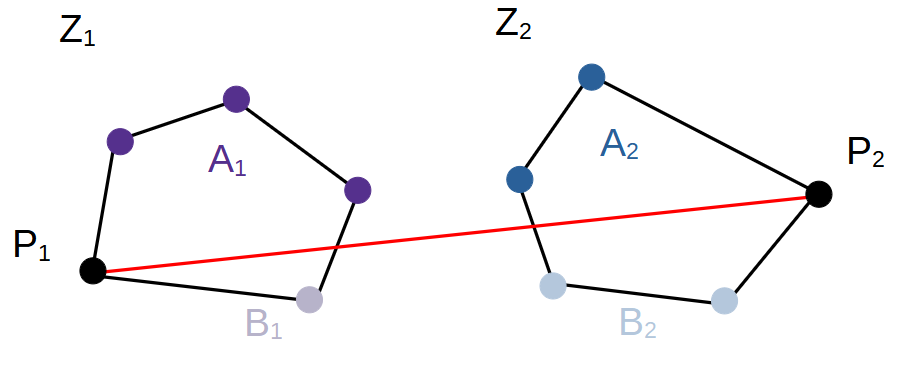
\includegraphics[scale=0.5]{data/zad75.png}
	\caption{Rysunek przedstawia przykładowe otoczki wejściowe oraz utworzone zbiory $A_i$, $B_i$ ($i \in \{1, 2\}$)}
	\label{fig:laczenieotoczek}
\end{figure}

Następnym krokiem jest utworzenie otoczki górnej oraz dolnej.
W tym celu zastosujemy algorytm Grahama bez sortowania 
wierzchołków dla obu
zbiorów: pod prostą $P_1P_2$ oraz nad prostą $P_1P_2$. 
Argumentem wejściowym do tak zmodyfikowanego algorytmu Grahama 
powinna być lista wierzchołków $P_2, A_2, A_1, P_1$
(w dokładnie takiej kolejności), w 
przypadku szukania otoczki górnej oraz $P_1, B_1, B_2, P_2$
(w dokładnie takiej kolejności) w przypadku
szukania otoczki dolnej.

Łączenie wyjściowych (dolnej i górnej) otoczek polega na 
doczepieniu do listy punktów otoczki dolnej listy punktów otoczki górnej.

\begin{algorithm}[H]
	\caption{Algorytm łączenia dwóch otoczek}
	\begin{algorithmic}[1]
		\Procedure{MergeConvexHulls}{$Z_1, Z_2$: zbiory wierzchołków}
		\State $P_1 \gets$ najmniejszy wierzchołek względem współrzędnej x w $Z_1$
		\State $P_2 \gets$ największy wierzchołek względem współrzędnej x w $Z_2$
		\State $A_i \gets \{(x, y) \in Z_i : (P_1, P_2, (x,y)) \text{ tworzą skręt w lewo}\}$, gdzie $i \in \{1, 2\}$
		\State $B_i \gets \{(x, y) \in Z_i : (P_1, P_2, (x,y)) \text{ tworzą skręt w prawo}\}$, gdzie $i \in \{1, 2\}$
		\State $A \gets \{P_2, A_2, A_1, P_1\}$ \Comment Kolejność ma znaczenie
		\State $B \gets \{P_1, B_1, B_2, P_2\}$ \Comment Kolejność ma znaczenie
		\State $O_A \gets$ \textsc{NoSortGraham($A$)}
		\State $O_B \gets$ \textsc{NoSortGraham($B$)}
		\State Usuń $P_1$ oraz $P_2$ z $O_A$ \Comment Nie chcemy duplikatów $P_1$ i $P_2$
		\State \Return $\{O_B, O_A\}$ \Comment Kolejność ma znaczenie
		\EndProcedure
		
		\Procedure{NoSortGraham}{$P$: zbiór punktów} \Comment Graham bez sortowania
		\State $S \gets \text{pusty stos}$
		\State $S$.Push($P[0]$)
		\State $S$.Push($P[1]$)
		\For {$k = 2,3, \dots, n-1$}
		\While{($S$.BelowTop(), $S$.Top(), $P[k]$) nie jest skrętem w lewo}
		\State $S$.Pop()
		\EndWhile
		\State $S$.Push($P[k]$)
		\EndFor
		\State \Return $S$
		\EndProcedure
	\end{algorithmic}
\end{algorithm}

Złożoność powyższego algorytmu wynosi $O(|Z_1| + |Z_2|)$.